\documentclass{article}
\usepackage[utf8]{inputenc}

\usepackage{graphicx}
\graphicspath{ {./images/} }

\title{Matrix Multiplication}
\author{Diaconescu Bogdan Florin}
\date{January 2020}

\begin{document}

\maketitle

\section{Problem statement}
Develop and implement a program to multiply 2 matrices
of size 1024x1024 using divide-et-impera.\\
The multiplication of matrices will be realized in a concurrent way using execu-
tors and the number of threads will be given by the number of available virtual
CPUs.

\section{Implementation/Solution}
Pentru rezolvarea problemei am creat 3 clase:
\begin{itemize}
    \item \textbf{Multiplier}: clasa care realizeaza inmultirea a 2 matrici pe un interval specificat.
        \begin{itemize}
            \item Cele 2 matrici sunt reprezentate de variabilele \textit{A[][]} si \textit{B[][]} \item \textit{size} reprezinta dimensiunea matricelor
            \item \textit{range} reprezinta intervalul matricelor pe care se executa inmultirea
            \item Am utilizat un zavor \textit{counterLock} folosit pentru accesul la contorul \textit{counter} al threadurilor care si-au incheiat sarcina.
            \item In functia \textit{run()} 
            \begin{itemize}
                \item Sunt parcurse cele 2 matrici in functie de intervalul specificat, sunt inmultite iar rezultatul este pus in matricea \textit{C[][]} din clasa \textit{Main}
                \item Dupa ce threadul si-a incheiat executia este blocat zavorul \textit{counterLock} pentru ca valoarea variabilei \textit{counter} sa nu fie modificata de alt thread
                \item se incrementeaza \textit{counter} si se elibereaza zavorul
            \end{itemize}
        \item Functia \textit{finished()} returneaza numarul de threaduri care si-au incheiat executia.
        \end{itemize}
    \item \textbf{MultiplicationExecutor} reprezinta clasa executor pentru multiplicarea matricelor. In functia \textit{run()} este creat threadul si este pus in executie prin apelarea metodei \textit{start()}.
    \item \textbf{MainClass}: functia ce contine metoda main().
        \begin{itemize}
            \item Aceasta are ca variabile cele 2 matrice, matricea rezultat \textit{C[][]}, precum si dimensiunea lor \textit{size = 1024} 
            \item In functia \textit{main()} 
            \begin{itemize}
                \item Sunt determinate numarul de procesoare virtuale disponibile \textit{workingThreads}
                \item Sunt generate random cele 2 matrice si sunt afisate
                \item Sunt impartite sarcinile in functie de numarul de threaduri disponibile
                \item este afisat rezultatul final.
            \end{itemize}
        \end{itemize}
\end{itemize}
\section{Experimental data}
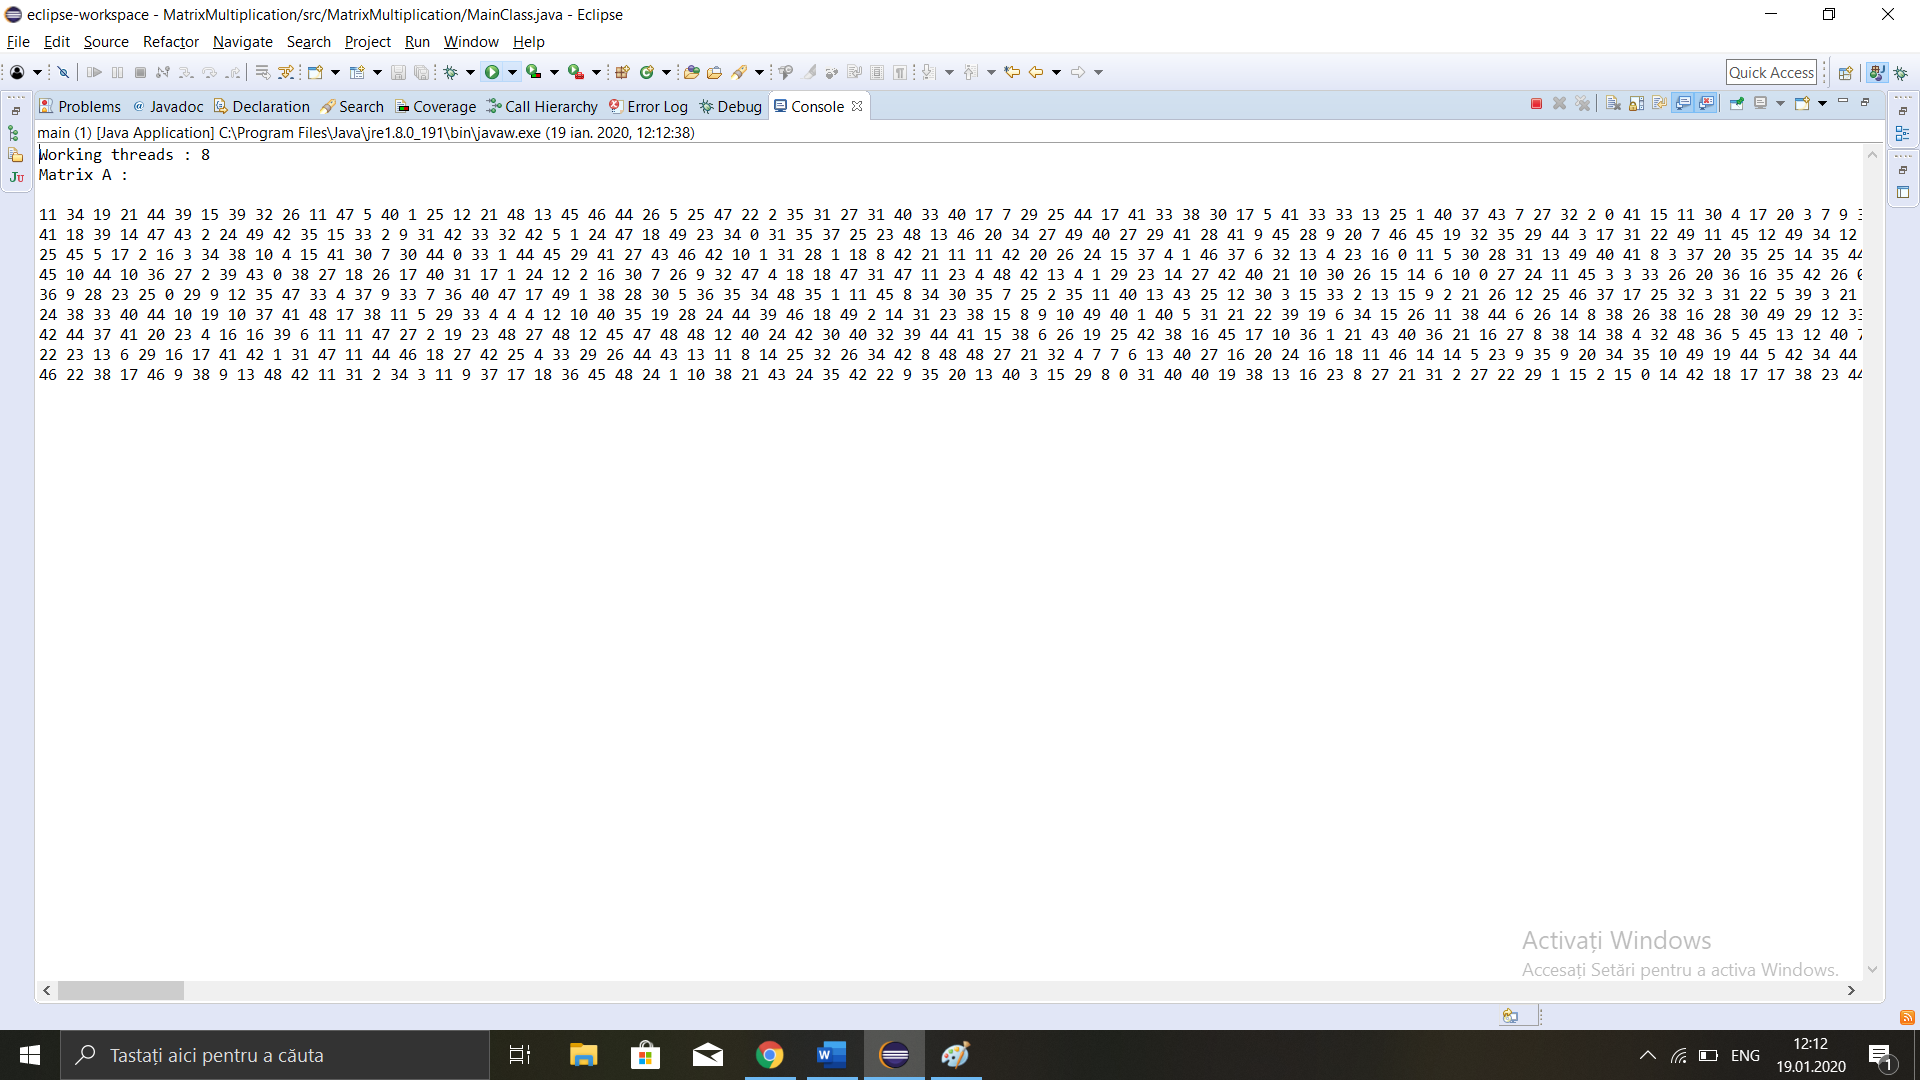
\includegraphics[scale=0.5]{MatrixMultiplication.png}
\section{Results \& Conclusions}
Am rezolvat problema inmultirii a 2 matrice prin divizarea lor pe mai multe intervale, inmultirea pe aceste intervale find facuta separat de catre un thread. Numarul threadurilor este egal cu numarul de procesoare virtuale disponibile, iar la final rezultatul final a fost pus in matricea C[][] si afisat.

\end{document}
